\documentclass[10pt, journal, compsoc]{IEEEtran}
\usepackage[utf8]{inputenc}
\usepackage{amsmath}
\usepackage{amsfonts}
\usepackage{amssymb}
\usepackage{graphicx}
\usepackage{subcaption}
\usepackage{algorithm}
\usepackage{algorithmicx}
\usepackage[noend]{algpseudocode}
\usepackage[left=2cm,right=2cm,top=2cm,bottom=2cm]{geometry}
\author{Tyrus~Cukavac (thc2125), Columbia University, Fu Foundation School of Engineering and Applied Science, Computer Science Department%
\thanks{Special thanks to Homayoon Beigi for n-phone model inspiration and recommendation to compare against monophone model.}}
\title{uRobo: An End-to-End Concatenative Speech Synthesis System}
\date{December 21, 2017}
\begin{document}
\maketitle
\begin{abstract}
This paper introduces uRobo, an open concatenative speech synthesis system built using the Kaldi framework for its Automated Speech Recognition layer and utilizing deep recurrent neural networks for target feature predictions in the unit selection stage. uRobo is an end-to-end system, meant to automate construction of a final model from raw data to synthesized speech, and to produce limited synthetic human speech from a small initial transcribed audio data set. Included target feature prediction models for uRobo were trained on ten hours of the LibriSpeech audio corpus comprising multiple female voices, while units used for concatenation during testing came from one of two data sets: one comprised of 10 hours of heterogenous speaker data, and another consisting of roughly 25 minutes of data from a single speaker. Moreover, uRobo is capable of unit selection at the triphone level (with diphone and monophone backoff) as well as the monophone level. We show that uRobo is able to produce intelligible voices with both of these models, but the triphone-diphone-monophone backoff architecture produces more intelligible and slightly smoother results.
\end{abstract}
\section{Introduction}
The generation of artificial, yet natural-sounding speech is one of the oldest problems in computer science. Although production of a general, intelligible synthetic voice is a worthy goal, there also exists a need to create voices which sound like a target speaker. This need is particularly acute in the domains of healthcare and media production. Many people who must have their voiceboxes removed for medical reasons such as cancer, often wish for the ability to re-create their orginal voice. Moreover, for film production companies, imperfect audio captured during filming force them to engage in time-intense and expensive audio recording sessions with their talent in order to meet production deadlines.\par
The largest challenge in replicating a given voice is often the lack of quality, annotated vocal data from the target voice. Film productions may only have twenty to forty-five minutes of provided audio from the desired speaker. And when recreating a voice for medical purposes, an engineer is unlikely to find that their potential users have maintained extensive, transcribed recordings of their everyday conversations.\par
To this end, uRobo attempts to create a new speech synthesis model that sounds similar to a target voice but does not necessarily require the hours and hours of training data needed to produce standard synthetic models.
\subsection{Existing Architectures}
State of the art text-to-speech architectures tend to follow one of three different approaches: a parametric approach, an end-to-end neural network approach, and a concatenative approach.\par
The parametric architecture essentially works to make predictions on durations of phonemes as well as the acoustic features necessary for synthesis. These acoustic features are then provided to a vocoder which synthesizes the sounds into waveforms.The parametric model described by Zen, et. al. utilizes an LSTM (Long Short Term Memory) RNN (Recurrent Neural Network) to make predictions of the above features.\cite{DBLP:journals/corr/ZenAEHS16} Although parametric models are resilient in the sense that they are capable of producing features for any desired frame (in comparison to other models that may be limited by the unit data collected during training), from a listener perspective the results are decidedly machine-like and lack a natural sound.\par
Neural networks have also found use outside of the parametric approach, and can in fact be used for end-to-end speech generation. The most recent state of the art architectures for text-to-speech synthesis make use of neural networks to generate pure waveform samples directly from input text. DeepMind's Wavenet uses dilated causal convolutional neural networks\cite{DBLP:journals/corr/ArikCCDGKLMRSS17}, and Baidu's Deep Voice passes inputs through layers of recurrent neural networks. Both of these approaches result in synthetic voices that human listeners seem to find more natural than previous approaches\cite{DBLP:journals/corr/OordDZSVGKSK16}, but require a great deal of computational power and time to train. Moreover, this area of study is still in relative infancy as opposed to other approaches, such as the concatenative, which have had more time to mature.\par
In contast to the other two methods, the concatenative approach to synthesis, as described by Hunt and Black, selects pre-existing units of audio from a database of annotated utterances, stitching these together and performing basic post-processing to create a final audio output\cite{Hunt:1996:USC:1256383.1256532}. The concatenative approach is often capable of yielding more natural-sounding results in than parametric models, due to its use of existing waveforms rather than the synthesis of new waveforms by a vocoder, which can result in noticeable  artifacting.\par
For the purposes of imitating a given speaker, the concatenative approach may seemingly yield the best of many worlds: taking less time and resources to train than an end-to-end neural network model while also being able to match actual phonetic level sounds from a given speaker. As a result, the uRobo system follows this architecture to synthesize speech, while also experimenting with extension of the selected units .  
\section{The Concatenative Approach}
The concatenative approach to synthesis is at its heart a dynamic programming problem. Given a database of units (pre-recorded waveforms, often with extracted acoustic features), the algorithm attempts to find a path/sequence of units corresponding to a given sequence of words/phonemes resulting in the minimum total cost value over all units. \par
\begin{equation}\overline{u}_1^n=min_{u_1,...,u_n}C(t_1^n,u_1^n)
\end{equation}
wherein $\overline{u}_1^n$ is the final sequence of $n$ units required for a new utterance that are selected by the algorithm. $u_x, x\in n$ is a given unit at index $x$ and $t_x, x\in n$ is a target "unit" or rather a representation of certain features that a unit at index $x$ should have. $C$ is a cost function over a sequence of units.\\	
The cost value per unit can be defined as a function of two separate costs. The target cost $C^t$, which is essentially a weighted sum of absolute differences between a target feature vector and a candidate unit's feature vector, as well as a concatenation cost $C^c$, which is the weighted sum of absolute differences between a candidate unit and a previous candidate.\par
\begin{equation}
C^t(t_i,u_i)=\sum_{j=1}^pw_j^t|t_{i_j}-u_{i_j}|
\end{equation}
\begin{equation}
C^c(u_{i-1},u_i)=\sum_{j=1}^qw_j^c|u_{i-1_j}-u_{i_j}|
\end{equation}
Where $p$ represents the number of features in the target feature vector and $q$ represents the number of features in the concatenation feature vectors of the two units. The cost for a given unit, then, is the sum of $C^c and C^t$. We can thus expand the cost of a sequence into the following equation:\par
\begin{equation}C(t_1^n,u_1^n)=\sum_{i=1}^nC^t(t_i,u_i)+ \sum_{i=1}^nC^c(u_{i-1},u_i)
\end{equation}\cite{Hunt:1996:USC:1256383.1256532}\par
Obviously calculating this for every possible path would be an intractable problem, therefore the Viterbi algorithm is used to find the minimum cost sequence. The problem can be visualized as a sparse matrix wherein each column corresponds to the set of candidate costs for a given unit. The first column of the matrix is initialized as the concatenation cost between the first unit and silence. In the remaining iterations, unit by unit, each candidate is compared against 1) the target feature vector and 2) all candidates for the previous unit. The minimum concatenation cost is selected as the final concatenation cost for that unit, and the previous unit candidate which resulted in that cost  is stored in a backtracking matrix.\par
\begin{algorithm}
\begin{algorithmic}[1]
\Function{VITERBI-UNIT-COSTS}{$t_1^n,u_1^n$}
\State{matrix $cost$}
\State{matrix $back$}
\For{each $u_{1_x}$ in $u_1$}
    \State{$cost_{1,x}=C^c($SIL$,u_1)$}
\EndFor
\For{each $u_{i}$ in $u_2^n$}
    \For{each $u_{i_x}$ in $u_i$}
        \State{$C^t(t_i,u_{i_x})$}
        \State{$C^c(u_{i_x})=\min C^c(u_{i-1},u_i{_x})$}
        \State{$b=$argmin $C^c(u_{i-1},u_i{_x})$}
        \State{$cost_{i,x}=C^t(t_i,u_{i_x})+C^c(u_{i_x}+cost_{i-1,b}$}
        \State{$back_{i,x}=b$}
     \EndFor
\EndFor
\Return{$cost,back$}
\EndFunction
\end{algorithmic}
\end{algorithm}
This final sequence of units i.e. selected waveforms, is recovered using a backtrace algorithm, then stitched together to create the final waveform representing a query utterance.
\section{uRobo Architecture}
The uRobo system is a concatenative system based on both monophones and/or triphones with diphone and monophone backoff, to be discussed in another section. To achieve this, the system is composed of four distinct layers, the output of which is fed into the next layer of the model, ultimately resulting in a synthesizer. First, the system needs to be able to decompose audio in a manner that features can be extracted for use in unit selection, and therefore requires a speech recognition system as the first step in preprocessing. Next, a system is required to analzye the raw output of the ASR in order to extract additional features and put them into a form that the target feature predicter can learn from. A model for predicting target features must then be trained on pre-processed data. Finally, a unit selection system using the viterbi algorithm and the previously extracted data can be used to acquire units and ultimately synthesize an audio file from text. The final system is built in Python, making extensive use of NumPy, as well as pysptk for secondary feature extraction.
\subsection{Speech Recognition System}
For automated speech recognition, the Kaldi ASR framework was utilized.\cite{Povey_ASRU2011} Kaldi has pre-built scripts that allow a user to train an ASR system on the LibriSpeech corpus\cite{unknown}, an open corpus that is the foundation of the data used by the uRobo concatenative synthesis system. Kaldi's training script for ASR downloads the LibriSpeech corpus as well as the language model files generated from an analysis of that corpus, i.e. vocabulary, phones, and a lexicon translating words to various phone sequences.\par
Kaldi then goes through all of the data, a total of 1000 hours, and builds triphone based alignment models utilizing HMM-GMMs and decision trees, extracting features such as MFCCs as well as performing multiple alignments on the data to improve each successive model.\par
With a final alignment model completed, the uRobo system can call kaldi scripts to perform forced alignment on the librispeech data. For the purposes of development and the experiments to follow, a subset of the clean training data of Librispeech, comprising 100 hours of audio data, as well as the clean test data, were aligned and output into a text format that specified a given utterance's timecode to specific phones. \par
Of particular use in the uRobo system was Kaldi's generation of an alignment lexicon, which provided additional contextual information for all of the possible/available phones, such as phone placement within the word. This became especially important for pre-selection of candidate units during the unit selection stage.
\subsection{Preprocessing}
Given properly aligned data from Kaldi's forced alignment, the uRobo preprocessor takes this output and extracts additional features, while also converting into a format more easily digestible by the neural network (in this case numpy arrays). The preprocessor takes librispeech audio data and converts it into wav format (for standardized feature extraction) as well as convert other Kaldi provided metrics and annotations for use in the training/synthesis stage. The preprocessor also allows for segmentation of the original data set by gender, speaker, and total duration.\par
Of key importance to the Librispeech model is the triphone/diphone/monophone chunking when analysing textual data. To this end, in order to train and utilize a target feature prediction model, a numerical index must be assigned to each monophone, diphone, and triphone respectively. Because modeling all possible triphones and diphones is virtually intractable, the existing utterances are first decomposed into diphones and triphones. Diphones and triphones that make up $1\%$ and $.1\%$ of the total data set respectively, are considered "representative" diphones or triphones and assigned a numerical index. A final index list combining monophone indices, with new numerical indices for the representative diphones and triphones is then created. (Note that this list of monophones, diphones, and triphones can later be used during preprocessing of other data to ensure uniformity of index assignment across different sets of utterances.)\par
With this list of mono-di-triphones, (hereafter referred to simply as "n-phones"), the utterances are then analyzed and chunked. For each phone $p_i$ in each utterance, the following triphone $p_i,p_{i+1},p_{i+2}$,is determined. If the triphone is representative (i.e. an index exists for it in the monophone-diphone-triphone dictionary previously extracted), the triphone's index is assigned to this chunk. If the triphone is not representative, however, the following diphone $p_i,p_{i+1}$ is determined instead. If it is representative, then an index is assigned to this chunk. If it is not, then the monophone is determined and its index is assigned to the phone.\par
The next phone to be chunked in this manner is the final phone in the current triphone ($p_{i+2}$) or diphone ($p_{i+1}$). This creates a single phone overlap for each chunk in an utterance. In the case of a monophone index being assigned, the following phone $p_{i+1}$ is chunked next.\par
Given the n-phone index representation of an utterance, features need to be extracted both for determining the target cost $C^t$ and the concatenation cost $C^c$. uRobo's target feature prediction model, discussed in the next subsection, attempts to predict acoustic features and compare against units in the database. Acoustic features selected, based on previous work in DNN target feature prediction, are a given n-phone's duration, energy, initial phone $f_0$ and final phone $f_0$. (Obviously in the case of monophones, initial phone $f_0$ and final phone $f_0$ are equivalent.) Energy in this instance is the sum of squared signal values divided by the duration of the total unit (for $n$ samples $s_{1...n}$, $\textrm{energy}=\frac{\sum_{j=1}^n s_j^2}{n}$).\cite{Jurafsky:2009:SLP:1214993}. Because the final synthesis will consist of overlapping phones, phone-level features remain the primary interest. In comparison to other models, which typically extract features on adjoining frames during concatenation\cite{a102c4924c19470ab180d278d2029de5}, uRobo's concatenation cost makes use of the existing target features for overlapping phones.\par
Because the features are meant to be fed as training output for a neural network, and given the wildly differing ranges of features, feature scaling must also occur in the pre-processing stage. Each feature is standardized against the mean and standard deviation over the utterances by any given speaker, so that each feature's final score is speaker independent. So for a target feature vector $t_{s}$ emitted by speaker $s$, $\hat{t}_s=\frac{t_s-\mu_s}{\sigma_s}$\cite{Beigi:2011:FSR:2124400}. In this manner, the target feature prediction model can be trained over significant amounts of data from different speakers while still being useful in predicting acoustic features for a single speaker.\par
For a given data set, feature extraction occurs over all monophones found in the source data as well, in order to provide for more phonetic coverage in the unit database. With the n-phone model alone, many phones will be incorporated into either tri-phones or di-phones. By extracting features for every existing unit at the phone level, more units are available to each of the initially identified monophones.
\subsection{Target Feature Prediction Using a Deep Recurrent Neural Network}
Hunt and Black present the general concept behind the Concatenative approach, but there is still the question of how to generate target features for computation of the target cost $C^t$. Much work has been done in this area, ranging from Festival's Multisyn system, which primarily utilizes linguistic features (phone, word, syllable boundaries, and accents)\cite{a102c4924c19470ab180d278d2029de5} as well as optional pitch contour and segment durations to create a target sequence of units that are then compared against the database. More recent research has begun to explore the potential of deep neural networks for predicting target features, learning both useful linguistic features and their association with desired acoustic features simultaneously. Merritt, et. al. utilized 5-6 layer feed forward DNNs to guide unit selection within the context of the Festival framework.\cite{7472658}.\par
For the uRobo architecture, a Recurrent Neural Network (RNN) model was adopted, inspired by that described by Fernandez, et. al. from the IBM Haifa Research Lab. The benefits of using a recurrent model are manifold, in particular the ability of RNNs to learn contextual information from given sequences. The base model consists of three stacked Bidirectional Long Short-Term memory (LSTM) layers.\cite{unknowndnn} For the purposes of this prototype, Tensorflow utilizing a Keras front-end was used to construct and train the neural mode.\cite{chollet2015keras} The input to the neural model consisted of indexes referencing n-phones. These were then translated to a neural embedding layer that was learned along with the phonetic-acoustic model. The uRobo model learns 32-dimensional embeddings for each given n-phone index. \par 
As per standard LSTM architecture, each n-phone embedding for a given utterance is then fed into a recurrent cell in the LSTM, the output of which was fed as input back into the recurrent cell (along with the next n-phone embedding). Because the layer is bidirectional, each of the n-phones are then input backwards through the recurrent pipeline (to acquire reverse context for each phone as well), with outputs at each stage of this sequence concatenated with the outputs of the forward layer. These final concatenated outputs (which are one-to-one with the phone inputs) are then used as sequential inputs into another bidirectional LSTM layer. The three Bidirectional LSTM layers output vectors of dimensions 67, 57, and 46 respectively.\cite{unknowndnn} A final dense layer is then distributed over the entire sequence, producing a 4-dimensional target feature vector for each given phone.\par
Each model is trained using the mean square error as the loss function. Although the model on which the predicter is based utilized standard stochastic gradient descent\cite{unknowndnn} for back propagation, initial training tests demonstrated slow, if any, convergence. Therefore for the purposes of our experiments, the RMSProp optimizer was employed.\par
\subsection{Unit Selection and Concatenation}
With a model capable of predicting target features, all that remains is to select audio units at the n-phone level to produce the final synthetic audio. For testing purposes, uRobo is capable of concatenating both n-phones or monophones, if so specified by the user.\par 
Given a sequence of words $w$ to synthesize, a sequence of $m$ n-phones $p_1^m$ is generated, using a naive and direct translation from word to phone sequence as provided by Kaldi's alignment lexicon. Given the high number of silence phones found within the audio data, adding silence was shown to have a detrimental effect on both runtime and fluency/intelligibility. Therefore silence phones were ignored in phone sequence generation. The phones are then chunked in a manner similar to initial preprocessing.\par 
With $p_1^m$, candidate pre-selection occurs to significantly reduce the unit search space for each n-phone. This is especially useful for data sets with many hours of audio, as the Viterbi algorithm utilized for unit selection runs in $O(n^3)$ time. Pre-selection in this instance follows a naive "phone to units" scheme, where for any given n-phone, the only possible candidate units are those that were classified as that specific n-phone during pre-processing. If no candidate units for an n-phone exist, the synthesizer splits the n-phone back into monophones, and selects candidate units from the monophone data that was also collected during pre-processing. Following candidate selection, the system uses the target feature prediction neural network to generate a sequence of target features for each phone.\par 
Costs are now calculated for each candidate unit as defined in section 2, with a few caveats. First, during the initialization of the cost matrix, a candidate unit's cost is not based on concatenation cost of the unit with silence ($C^c($SIL$u_1$)). Instead, the cost is purely a function the candidate unit's target cost.\par
Moreover, to encourage selection of overlapping units, a concatenation cost of 0 is applied if two adjacent candidate units do in fact overlap in the source data. Finally, no weights were applied, giving (relatively) equal representation to the different comparison features used to determine cost.\par
When final units are selected from the data, each of the units is concatenized, albeit with the last phone of a given unit overlapping with the first phone of the next unit. To make transitions smoother and avoid the unpleasant effect of hearing multiple voices at once, a logarithmic cross fade is applied at the time of the join, i.e. the first sample of the final phone in the previous unit. Note that if a monophone is followed by another monophone or the model solely uses monophones as units, these units are directly concatenated together. A final wav file is then exported by the system.
\section{Experiment Setup}
\subsection{The Corpus}
As previously mentioned, much of the difficulty in speech synthesis lies in a lack of substantial and usable training data. Many of the corpora used by large corporations incorporate many hours of audio data recorded by professional voice actors, and are not freely available to the public. The open Librispeech corpus\cite{unknown} aims to fill this gap by formatting and segmenting data from the LibriVox project, providing thousands of hours of transcribed audio data for use in speech tasks. Unfortunately, each speaker in the corpus tends to only contribute a maximum of around 30 minutes of audio to the overall project, meaning any attempts at making use of this data for a text-to-speech model will either need to compose units from varied voices or from a very limited data set of audio.\par
\subsection{Utterance Synthesis and Metrics}
Both of the above approaches were used in the experiments. A set of ten utterances were generated. Each word contained one to five syllables, in increasing order. The five sentences likewise began simply but became progressively more difficult to pronounce. The utterances were generated by synthesizers using two different data sets. One utilized a single female speaker from the LibriSpeech training corpus, comprising roughly 25 minutes of audio spoken. The other, to test the viability of "found data" or combinations of pre-existing but sonically distinct data, used ten hours of total audio spoken by multiple female readers from the corpus. To test the variation between n-phone and pure monophone unit selection, two different synthesizers were built from the single speaker data: one concatenating n-phones while another worked with solely with monophones. This resulted in 3 different synthetic voices. All of the test voices utilized the same target feature prediction neural model, which was trained over twenty epochs on ten hours of female speaker data.\par 
The target words/sentences themselves were selected from the test set of the Librispeech corpus. This assured, at least at the sentence level, that the utterances would be "unseen" by any of the voices. This selection had the added benefit of providing pre-recorded human audio so that a control group could be used as a baseline comparison for the desired metrics. \par
The generated and control audio was judged by a blind sampling of five distinct Mechanical Turk workers per utterance. Each judged an individual audio file based on three metrics: the intelligibility of the utterance, how human it sounded, and the smoothness of the utterance.\par
Although a similarity test comparing the synthesized audio with the original speaker would provide insight into uRobo's effectiveness at creating a voice similar to a target, this would likely be better performed with a new corpus comprising more than thirty minutes of data from a single speaker. As it is, synthesizing speech from text previously uttered by the initial speaker is clearly similar to the original utterances of the speaker, due in part to the zero cost concatenation between overlapping n-phones. Essentially it is a close re-creation of the source utterance, which would not provide any useful metric. Attempts to alleviate this by removing certain utterances would serve to reduce the already limited phonetic coverage. Certain n-phones and monophones, in fact, lack any unit representation, even with the complete 25 minutes of audio. As a result, all units from the source data need to be utilized to provide adequate phonetic coverage.
\section{Results}
Figure 1 shows the results of the vocal quality survery given over Mechanical Turk. A total of 28 different workers participated in the survey and each judged an average of roughly 7 voice samples. The top four workers each listened to more than 27 of the 40 samples provided. \par
The results show the obvious dominance of the control (human) voice, which is to be expected. Similarly, the single speaker voice utilizing the n-phone model also shows significant advantages over both the multi-speaker voice and the monophone only single speaker voice.\par
\begin{figure}[h]
\caption{In the figure below, "c" represents the control human voice, "t10f" represents the voice selecting from ten hours of multi-speaker data, "ts39" refers specifically to the single speaker voice (speaker 39 in LibriSpeech) and "ts39\_m" represents its monophone variant.}
\centering
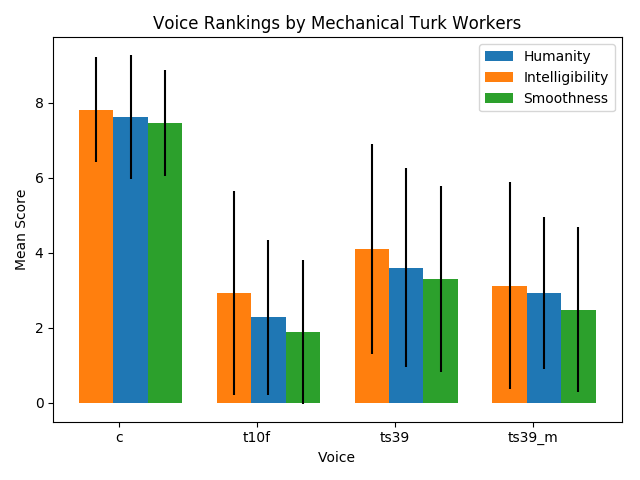
\includegraphics[scale=.5]{../experiments/results/all_voices_results.png}
\end{figure}
The high variability in the answers as demonstrated by the standard deviation line showcases a similar trend, but also the difficulty in accurately measuring the effectiveness of a given voice. That said, clear trends do emerge, and the results show the superiority of a triphone model with backoff over a pure monophone model.\par
Analysis was also made of the single speaker model's performance with regards to increasing complexity of words and sentences. Figures 2 and 3 show line graphs demonstrating the voice's performance as the number of syllables and words increase respectively. Unfortunately, there is a significant decline as the complexity of both sentences and words increases, despite promising performance with simpler words and sentences. Future efforts towards the model, discussed in the next section, will look to increase these scores.
\begin{figure}[h]
    \caption{}
    \centering
    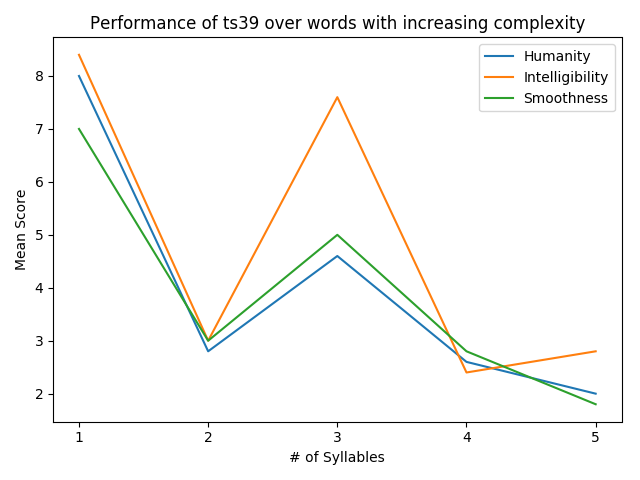
\includegraphics[width=1\linewidth]{../experiments/results/ts39_word_results.png}
\end{figure}
\begin{figure}[h]
    \caption{}
    \centering
    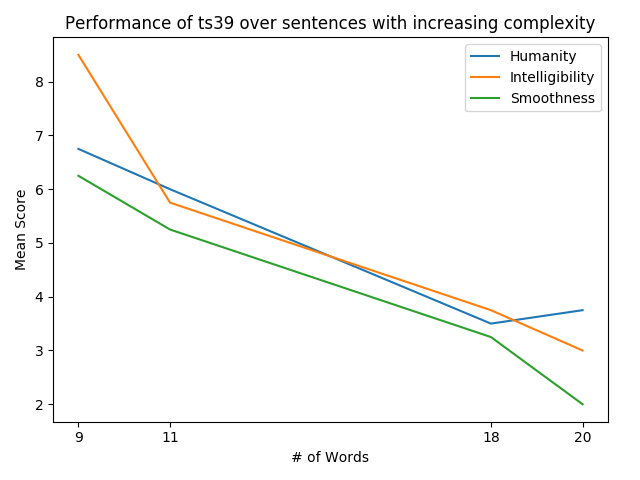
\includegraphics[width=1\linewidth]{../experiments/results/ts39_sent_results.png}
\end{figure}
\section{Conclusions and Avenues for Future Work}
There are a number of areas for improvement in the current architecture. In particular, with regards to being able to "re-synthesize" the original audio given a string of text. The phonetic pronunciation of a given sentence is provided without respect to the placement of silences. The original LibriSpeech data set is rife with silences between some words but not others, and also at the beginning and end of each utterance. uRobo currently uses the alignment lexicon to translate a word into its phonetic pronunciation, without regard to any intermediate silences that might occur. For a future version of uRobo, it may be worthwhile to experiment with a sequence to sequence model or HMM that is capable of learning when and where silences should be placed. This might allow for better unit selection, particularly with low resource speakers that may have many triphone and diphone sequences that are dependent on the silences between words. \par
A great deal of improvement could also be made in the area of post-processing and smoothing out the actual concatenations, perhaps by some form of pitch-shifting over the course of a given join, and even possibly some pitch normalization over an entire final sequence of synthesized audio.\par
Additionally, multiple other experiments may be useful in determining the viability of the uRobo model in single speaker voice simulation. Although the scope of this current project focused specifically on thirty minutes or less of a single speaker's data, it would be interesting to compare current results with a significantly larger single speaker corpus, possibly as a means of tuning hyperparameters for the neural model and experimentation of different feature sets for calculating concatenation and target cost.\par
On the whole, uRobo demonstrated relatively intelligible and human-sounding synthetic speech from a limited source data set. Unfortunately, the amount of data does curtail the robustness of the system. Further experimentation with larger data sets is required to effectively test the limits of the system and work on tuning the underlying models. \bibliographystyle{IEEEtran}
\bibliography{thc2125_paper}

\end{document}
